\documentclass[twocolumn,10pt]{ltjsarticle}

\usepackage[top=15mm,bottom=15mm,left=20mm,right=20mm,columnsep=10mm]{geometry}
\usepackage[haranoaji,nfssonly]{luatexja-preset}
\usepackage{graphicx}
\usepackage{titlesec}
\usepackage{url}

\usepackage{multirow}    % セル結合用
\usepackage{tabularx}    % 表用&カラムサイズ指定

%% カラムサイズの指定用 %%
\newcolumntype{C}[1]{>{\centering\arraybackslash}p{#1}}
\newcolumntype{L}[1]{>{\raggedright\arraybackslash}p{#1}}
\newcolumntype{R}[1]{>{\raggedleft\arraybackslash}p{#1}}

\title{【実験】BOS\_2016の周期分析結果の比較}
\author{山下 尚彦}
\date{\today}

\begin{document}
\maketitle

\section{はじめに}
本研究メモでは, 組織内ネットワークへの侵害活動を観測したデータセット「動的活動観測2016(BOS\_2016)」\cite{マルウェア対策研42:online}をLomb-Scargleピリオドグラムで周期分析した結果を, BOS\_2016について報告した論文\cite{weko_175829_1}との比較について述べる. 

\section{BOS2016について}
本章では, 実験に使用するデータセットBOS\_2016の概要について説明する. 

本研究の実験で使用するデータセットBOS\_2016は, 総務省実証事業「サイバー攻撃解析・防御モデル実践演習の実証実験の請負」で実施され, 研究者コミュニティから提供された組織内ネットワークへの侵害活動を動的に観測したデータセットである. マルウェア検体のハッシュ値情報や, 通信観測データ, プロセス観測データの他に, Windowsのイベントログやファイアウォールのログがデータセットとして提供されている. 

データセットには, マルウェアの動作が確認されC2サーバと正常に通信が発生して攻撃の観測ができた事例(Case e04)やC2サーバへのSYNパケットのみ送信した事例(Case e12, e20), C2サーバとの通信が確認されなかった事例(Case e70, e435), また, 動作が確認されなかった事例(Case e43)の観測データやログなどが記録されている(表\ref{tab:bos2016}). 

\begin{table}[htbp]
    \centering
    \caption{BOS\_2016の検体の挙動と通信について}

    \begin{tabular}{C{20mm}L{15mm}L{30mm}}
        %% カラム名 %%
        \hline
        Case & 挙動 & 通信 \\
        \hline \hline
        %% データ %%
        e04 & 動作 & 攻撃活動を観測 \\ \hline
        e12\par e20 & 動作 & C2サーバとの通信が成立しない(403, 404, 503) \\ \hline
        e43 & 実行不可 & 通信発生せず \\ \hline
        e70\par e435 & 動作 & C2サーバへSYNパケットのみ送信 \\
        \hline
    \end{tabular}

    \label{tab:bos2016}
\end{table}

\section{実験}
本章ではBOS\_2016のうち, 周期分析したデータと実験の条件について述べる. 

\subsection{周期分析する事例}
動的活動観測環境でマルウェアの検体を実行した機器のうち, e04はマルウェアが動作し実際に攻撃を観測したため, 通信観測データが提供されていなかった. よって, 実験ではe12, e20, e43, e70, e435の通信観測データと観測環境内で観測された通常の通信を含む全ての通信観測データを用いる. 

\subsection{実験条件}
通信観測データを1日ごとに分割してLomb-Scargleピリオドグラムで解析する. また, Lomb-Scargleピリオドグラムで解析した結果, 周期的である確率が90\%以上である信号を周期性のある通信とする.

\section{結果}
本章では, 通信観測データの周期分析実験の結果について述べる. なお, 本研究メモではマルウェア検体が動作しC2サーバとのTCPコネクションを確立したが, HTTPのステータスコードが403(Forbidden),404(Not Found), 503(Service Unavailable)などでC2サーバとの通信が成立しなかったe12とe20と, マルウェアが活動しTCP SYNパケットをC2サーバに送信したが, TCPコネクションを確立できなかったe70, e435の解析結果について記述する. 

表\ref{tab:e12}から表\ref{tab:e435}は, e12とe20, e70, e435の通信観測データを1日ごとに解析し, 送信元IP数(SRC), 送信元と受信先IPペア数(PAIR), 周期的である確率が99.9\%以上ある通信を行ったIPアドレスのペア数をまとめた表である. また, 表\ref{tab:e12_ip}, \ref{tab:e43_ip}, \ref{tab:e70_ip}はそれぞれの観測データで周期性を検出した通信の受信先IPアドレスの表である. 

図\ref{fig:e12_result}と図\ref{fig:e43_result}, 図\ref{fig:e70_result}のC2サーバとの通信回数とLomb-Scargleピリオドグラムによる解析結果のグラフである. ただし, e70は周期性のある通信を複数検出したため, C2サーバとの通信のみを記載する. 

\begin{table}[htbp]
    \centering
    \caption{e12の実験結果}

    \begin{tabular}{c||llllll}
        %% カラム名 %%
        \hline
        DATE & SRC & PAIR & 95\% & 99\% & 99.9\% \\
        \hline \hline
        %% データ %%
        20160212  & 21 & 42 & 2 & 0 & 0 \\
        20160213  & 5  & 8  & 0 & 0 & 0 \\
        20160215  & 8  & 14 & 0 & 0 & 0 \\
        20160216  & 4  & 6  & 0 & 0 & 0 \\
        \hline
    \end{tabular}
    \label{tab:e12}
\end{table}

\begin{table}[htbp]
    \centering
    \caption{e20の実験結果}

    \begin{tabular}{c||llllll}
        %% カラム名 %%
        \hline
        DATE & SRC & PAIR & 95\% & 99\% & 99.9\% \\
        \hline \hline
        %% データ %%
        20160215  & 14 & 27 & 0 & 0 & 0 \\
        20160216  & 5  & 8  & 0 & 0 & 0 \\
        20160217  & 5  & 8  & 0 & 0 & 0 \\
        20160218  & 8  & 15 & 0 & 0 & 0 \\
        \hline
    \end{tabular}
    \label{tab:e20}
\end{table}

\begin{table}[htbp]
    \centering
    \caption{e70の実験結果}

    \begin{tabular}{c||llllll}
        %% カラム名 %%
        \hline
        DATE & SRC & PAIR & 95\% & 99\% & 99.9\% \\
        \hline \hline
        %% データ %%
        20160215  & 16 & 34 & 6  & 4  & 3 \\
        20160216  & 7  & 15 & 10 & 10 & 5 \\
        20160217  & 12 & 25 & 6  & 6  & 3 \\
        20160218  & 7  & 16 & 7  & 7  & 6 \\
        \hline
    \end{tabular}
    \label{tab:e70}
\end{table}

\begin{table}[htbp]
    \centering
    \caption{e435の実験結果}

    \begin{tabular}{c||llllll}
        %% カラム名 %%
        \hline
        DATE & SRC & PAIR & 95\% & 99\% & 99.9\% \\
        \hline \hline
        %% データ %%
        20160328  & 16 & 31 & 0 & 0 & 0 \\
        20160329  & 2  & 3  & 0 & 0 & 0 \\
        20160330  & 5  & 9  & 0 & 0 & 0 \\
        \hline
    \end{tabular}
    
    \label{tab:e435}
\end{table}

\begin{table}[htbp]
    \centering
    \caption{e12で周期的な通信を示した受信先IPアドレス}

    \begin{tabular}{|c||c|l|}
        \hline
        DATE & PERIODIC & IP ADDRESS \\
        \hline \hline

        20160212 & 95.0\% & \begin{tabular}{l}
                               \ast\ast\ast.79.197.250
                            \end{tabular} \\ \hline
    \end{tabular}

    \label{tab:e12_ip}
\end{table}

\begin{table}[htbp]
    \centering
    \caption{e43で周期的な通信を示した受信先IPアドレス}

    \begin{tabular}{|c||c|l|}
        \hline
        DATE & PERIODIC & IP ADDRESS \\
        \hline \hline

        20160216 & 95.0\% & \begin{tabular}{l}
                               \ast\ast\ast.44.155.27
                            \end{tabular} \\ \hline
    \end{tabular}

    \label{tab:e43_ip}
\end{table}

\begin{table}[htbp]
    \centering
    \caption{e70で周期的な通信を示した受信先IPアドレス}

    \begin{tabular}{|c||c|l|}
        \hline
        DATE & PERIODIC & IP ADDRESS \\
        \hline \hline

        20160215 & 95.0\% & \begin{tabular}{l}
                               \ast\ast\ast.44.155.27
                            \end{tabular}       \\ \cline{2-3}
                 & 99.0\% & \begin{tabular}{l}
                               \ast\ast\ast.165.83.176
                            \end{tabular}       \\ \cline{2-3}
                 & 99.9\% & \begin{tabular}{l}
                               \ast\ast\ast.32.101.160  \\
                               \ast\ast\ast.106.20.192
                            \end{tabular}       \\ \hline
        20160216 & 99.0\% & \begin{tabular}{l}
                               \ast\ast\ast.106.149.145 \\
                               \ast\ast\ast.106.20.192
                            \end{tabular}       \\ \cline{2-3}
                 & 99.9\% & \begin{tabular}{l}
                               \ast\ast\ast.32.101.160  \\
                               \ast\ast\ast.165.83.176  \\
                               \ast\ast\ast.21.181.152  \\
                               \ast\ast\ast.208.153.9   \\
                            \end{tabular}       \\ \hline
        20160217 & 99.0\% & \begin{tabular}{l}
                               \ast\ast\ast.106.149.145 \\
                               \ast\ast\ast.106.253.18
                            \end{tabular}       \\ \cline{2-3}
                 & 99.9\% & \begin{tabular}{l}
                               \ast\ast\ast.165.83.176  \\
                               \ast\ast\ast.106.20.192
                            \end{tabular}       \\ \hline
        20160218 & 99.0\% & \begin{tabular}{l}
                               \ast\ast\ast.106.20.192
                            \end{tabular}       \\ \cline{2-3}
                 & 99.9\% & \begin{tabular}{l}
                               \ast\ast\ast.165.83.176  \\
                               \ast\ast\ast.21.181.152  \\
                               \ast\ast\ast.208.153.9   \\
                               \ast\ast\ast.106.149.145
                            \end{tabular}       \\ \hline
    \end{tabular}

    \label{tab:e70_ip}
\end{table}

\begin{figure}[htbp]
    \centering

    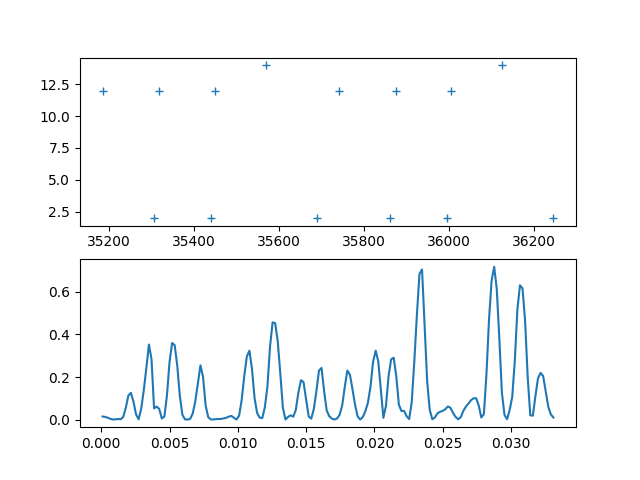
\includegraphics[width=7.5cm]{images/【実験】BOS_2016の周期分析結果の比較/e12.png}

    \caption{e12の通信回数と解析結果}
    \label{fig:e12_result}
\end{figure}

\begin{figure}[htbp]
    \centering

    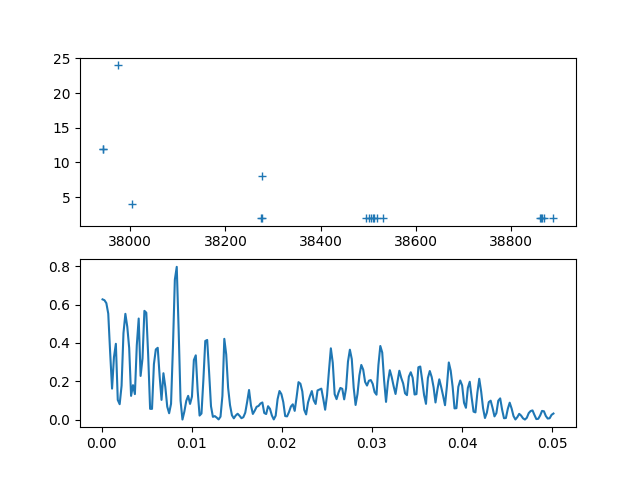
\includegraphics[width=7.5cm]{images/【実験】BOS_2016の周期分析結果の比較/e43.png}

    \caption{e43の通信回数と解析結果}
    \label{fig:e43_result}
\end{figure}

\begin{figure}[htbp]
    \centering

    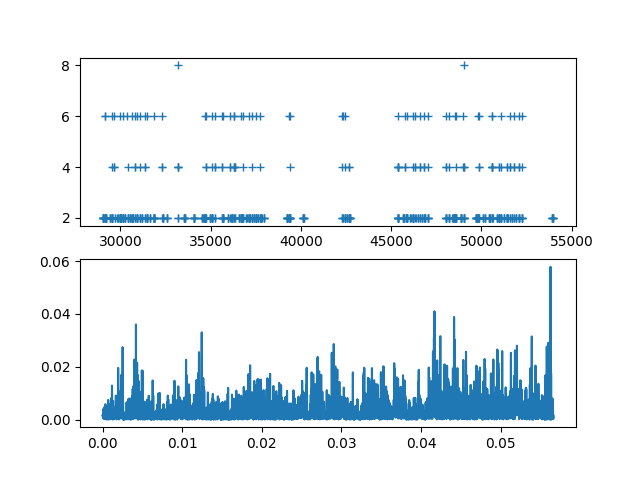
\includegraphics[width=7.5cm]{images/【実験】BOS_2016の周期分析結果の比較/e70.png}

    \caption{e70の通信回数と解析結果}
    \label{fig:e70_result}
\end{figure}

\section{考察}
本章では, 実験結果を寺田らがデータセットBOS\_2016について報告した内容\cite{weko_175829_1}と比較して考察する. 

寺田らの報告によると, C2サーバとのTCPコネクションを確立できたが, C2サーバとの通信が成立しなかったe12とe20のC2サーバのIPアドレスは, e12は\ast\ast\ast.56.81.119と\ast\ast\ast.76.86.155の2つで, e20は\ast\ast\ast.81.81.137と判明した. また, マルウェアが動作しC2サーバにTCP SYNパケットを送信できたが, TCPコネクションを確立できなかったe70とe435のC2サーバのIPアドレスはそれぞれ\ast\ast\ast.106.20.192と\ast\ast\ast.24.93.253である. 

今回の実験結果では, e70のケースでC2サーバとの周期的な通信を検出できたが, それ以外の事例ではC2サーバとの通信を検出することができなかった. e20とe435に至っては周期的な通信自体を発見することができなかった. これはデータ処理の際に, 記録されている通信時間をナノ秒から秒に変換されていたことが原因と考えられる. e12を例にすると, 図\ref{fig:e12_result}上部の通信時間と通信回数の関係を表したグラフから1秒間に2回や12回通信していたことが分かるが, 本来であれば通信を行った1回ごとのデータを解析する必要があるため, 正しく周期分析を行えていなかったと考えられる. 

\section{おわりに}
本研究メモでは, データセットBOS\_2016を解析した結果と, BOS\_2016について報告した論文の内容と比較して判明した問題点などについて述べた. 

報告論文と比較した結果, 今回の実験で検出した周期的な通信のうちC2サーバとの通信を検出できたのはe70の事例のみであった. これは, 通信時間の粒度が低く, 1秒間に複数回通信を行っていたというデータで周期分析したことが原因と考えられるため, 次回の実験時にはこの問題点を解決したいと思う. 

\bibliographystyle{junsrt}
\bibliography{DB}
\end{document}